\documentclass[twoside]{article}
\input{ISC18-english.sty}
\usepackage{graphicx}
%%%%%%%%%%%%%%%%%%%%%%%%%%%%  Make sure to compile twice for proper cross-references. %%%%%%%%%%%%%%%%%%%%%%%
%%%%%%% For proper display of references, compile the document twice. %%%%%%%%%%%%%%%%%%%%% 
%%%%%%%%%%%%%%% If using TeX Live, compile using pdflatex command %%%%%%%%%%%%%%%%%%%%%%%
\begin{document}
\thispagestyle{empty}
%%%%%%%%%%%%%%%%% Article title header  %%%%%%%%%%%%%%%%%%%%
\fancyhead[LE]{Mahalanobis Weighted Multivariate Normal Distribution}
%%%%%%%%%%%%%%%%% Article authors header   %%%%%%%%%%%%%%%%%%%%
\fancyhead[RO]{Fatemeh Shahsanaei}
\begin{center}
{
\includegraphics [height=25mm, width=150.3mm] {Images/isc18E}} \\
\vspace*{-1.8cm}
%\begin{center}
%\color{blue} 
%{\hspace{0.1cm}\rule{\textwidth}{1mm}}\\
%\end{center}
\vspace*{4cm}
%%%%%%%%%%%%%%%%% Article title  %%%%%%%%%%%%%%%%%%%%
{\Large \bf On a Novel Weighted Multivariate Normal Distribution Using Mahalanobis Distance}\\
%%%%%%%%%%%%%%%%% Article authors and affiliations %%%%%%%%%%%%%%%%%%%%
{\bf
Fatemeh Shahsanaei \footnote{{\bf Corresponding Authur :} {\tt f.shahsanai@scu.ac.ir }} \\
Department of Statistics, Shahid Chamran University of Ahvaz, Iran }
\end{center}
\rule{\textwidth}{0.2mm}\\
%%%%%%%%%%%%%%%%% Article abstract  %%%%%%%%%%%%%%%%%%%%
\noindent{\bf Abstract:}\\
	The standard Multivariate Normal distribution is inherently unimodal and concentrates its probability mass at the mean, making it inadequate for modeling non-centralized or ring-shaped data. To address this limitation, we introduce the Mahalanobis-Weighted Multivariate Normal Distribution. By employing the squared Mahalanobis distance as a weighting function, the Mahalanobis-Weighted Multivariate Normal Distribution forces the central density to exactly zero, creating a topological ``hole effect'' without introducing any additional parameters. Compared to complex alternatives like Gaussian Mixture Models, the Mahalanobis-Weighted Multivariate Normal Distribution offers a strictly parsimonious and mathematically elegant solution. Simulation studies demonstrate its superior performance and computational efficiency in fitting crater-like data topologies, with broad applications in medical imaging, urban planning, and ecology.
 
\noindent{\bf Keywords:} 
Weighted Distribution, Multivariate Normal Distribution, Mahalanobis Distance, Hole Effect \\
\noindent{\bf Mathematics Subject Classification (2010):} $\rm 62H05$, $\rm 60E05$, $\rm 62E15$. \\
\hspace{1cm}\rule{\textwidth}{0.2mm}\\
%%%%%%%%%%%%%%
\section{Introduction}
Motivated by the need to model complex, non-centralized data structures, this paper explores the limitations of traditional centralized distributions and proposes a novel alternative. The standard Multivariate Normal (MVN) distribution, despite its mathematical tractability and widespread use in statistical learning, is strictly unimodal. Its maximum probability density is heavily concentrated at the mean vector $\boldsymbol{\mu}$. This inherent characteristic severely limits its flexibility when analyzing real-world phenomena that naturally exhibit a crater-like topology or a ``hole effect,'' where the probability mass at the center is negligible or exactly zero.

To overcome the rigid structural limitations of standard probability models, the foundational concept of \textit{weighted distributions} was initially conceptualized by \cite{Fisher1934} and subsequently formalized and generalized by \cite{rao1965}. Weighted distributions provide a rigorous mathematical framework for adjusting baseline probabilities to account for weighted sampling. \cite{patil1978} extensively demonstrated the utility of these distributions in ecology, forestry, and spatial data analysis. Since then, various structural modifications to the MVN have been developed in the literature to increase its flexibility. A prominent example is the multivariate skew-normal distribution introduced by \cite{azzalini1985}, which successfully models asymmetric data. However, systematically generating a symmetric, crater-like density where the central probability mass is exactly evacuated remains structurally challenging.

Traditionally, modeling such radially distributed topologies requires complex statistical architectures, such as Gaussian Mixture Models (GMMs) or non-linear manifold learning techniques (\citet{mclachlan2000}). While effective, these methods inherently suffer from over-parameterization, increased computational overhead, and susceptibility to local optima during the parameter estimation process. The necessity for a parsimonious, mathematically tractable model is evident across various scientific domains:
\begin{enumerate}
	\item \textbf{Medical Imaging and Anomaly Detection:} Identifying irregular structures, such as tumors with necrotic (dead) cores (e.g., Glioblastoma), requires models capable of capturing an active outer tissue ring surrounding an empty center.
	\item \textbf{Urban Planning and Spatial Modeling:} The ``urban donut effect'' describes the hollowing out of city centers due to population migration to the suburbs, leaving a concentrated ring of population density around a sparse core.
	\item \textbf{Ecology and Biological Clustering:} Certain growth patterns, such as ``fairy rings'' formed by fungi or specific bacterial colonies, naturally exhibit circular spatial distributions that centralized models fail to capture accurately.
\end{enumerate}

To directly address this topological challenge with strict structural parsimony, we introduce the \textit{Mahalanobis-Weighted Multivariate Normal Distribution (MWMND)}. By utilizing the squared Mahalanobis distance (\cite{mahalanobis1936}) as a natural weighting mechanism, we systematically penalize probabilities near the mean center, effectively driving the density at $\boldsymbol{\mu}$ to zero. This geometric transformation radially redistributes the probability mass without introducing any additional parameters beyond those of the base MVN ($p$, $\boldsymbol{\mu}$, and $\boldsymbol{\Sigma}$). Consequently, the MWMND emerges as a highly robust, elegant, and parsimonious alternative for modeling scattered spatial phenomena and ring-shaped multidimensional data structures.

\section{The Mahalanobis-Weighted Multivariate Normal Distribution (MWMND)}

Let $\mathbf{X}$ be a $p$-dimensional random vector following a standard Multivariate Normal distribution, denoted as $\mathbf{X} \sim N_p(\boldsymbol{\mu}, \boldsymbol{\Sigma})$, where $\boldsymbol{\mu}$ is the mean vector and $\boldsymbol{\Sigma}$ is the positive-definite covariance matrix. The baseline probability density function (PDF) is given by:
\begin{equation}
	f_0(\mathbf{x}) = \frac{1}{(2\pi)^{p/2} |\boldsymbol{\Sigma}|^{1/2}} \exp\left(-\frac{1}{2} (\mathbf{x} - \boldsymbol{\mu})^T \boldsymbol{\Sigma}^{-1} (\mathbf{x} - \boldsymbol{\mu})\right)
\end{equation}

We define the weight function $w(\mathbf{x})$ as the squared Mahalanobis distance between $\mathbf{x}$ and $\boldsymbol{\mu}$:
\begin{equation}
	w(\mathbf{x}) = (\mathbf{x} - \boldsymbol{\mu})^T \boldsymbol{\Sigma}^{-1} (\mathbf{x} - \boldsymbol{\mu})
\end{equation}

Since $w(\mathbf{X})$ follows a Chi-square distribution with $p$ degrees of freedom ($\chi^2_p$), its expected value is exactly $p$:
\begin{equation}
	E[w(\mathbf{X})] = p
\end{equation}

The PDF of the proposed MWMND is obtained by weighting the baseline MVN density:
\begin{equation}
	f_w(\mathbf{x}) = \frac{w(\mathbf{x}) f_0(\mathbf{x})}{E[w(\mathbf{X})]}
\end{equation}

Substituting the components yields the explicit density function of the MWMND:
\begin{equation}
	f_w(\mathbf{x}) = \frac{(\mathbf{x} - \boldsymbol{\mu})^T \boldsymbol{\Sigma}^{-1} (\mathbf{x} - \boldsymbol{\mu})}{p (2\pi)^{p/2} |\boldsymbol{\Sigma}|^{1/2}} \exp\left(-\frac{1}{2} (\mathbf{x} - \boldsymbol{\mu})^T \boldsymbol{\Sigma}^{-1} (\mathbf{x} - \boldsymbol{\mu})\right)
\end{equation}

Geometrically, as $\mathbf{x} \to \boldsymbol{\mu}$, the Mahalanobis distance approaches zero, forcing $f_w(\mathbf{\mu}) = 0$. This guarantees a crater-like topology where the maximum density is distributed along an elliptical contour surrounding the mean, effectively capturing the "hole effect".
To provide a clear intuitive understanding of the topological transformation induced by this weighting mechanism, Figure~\ref{fig:mwmnd_3d_comparison} visualizes the probability density function of the proposed MWMND alongside the standard Multivariate Normal (MVN) distribution for a bivariate case ($p=2$) with standard parameters ($\boldsymbol{\mu} = \mathbf{0}$, $\boldsymbol{\Sigma} = \mathbf{I}$).

\begin{figure}[H]
	\centering
	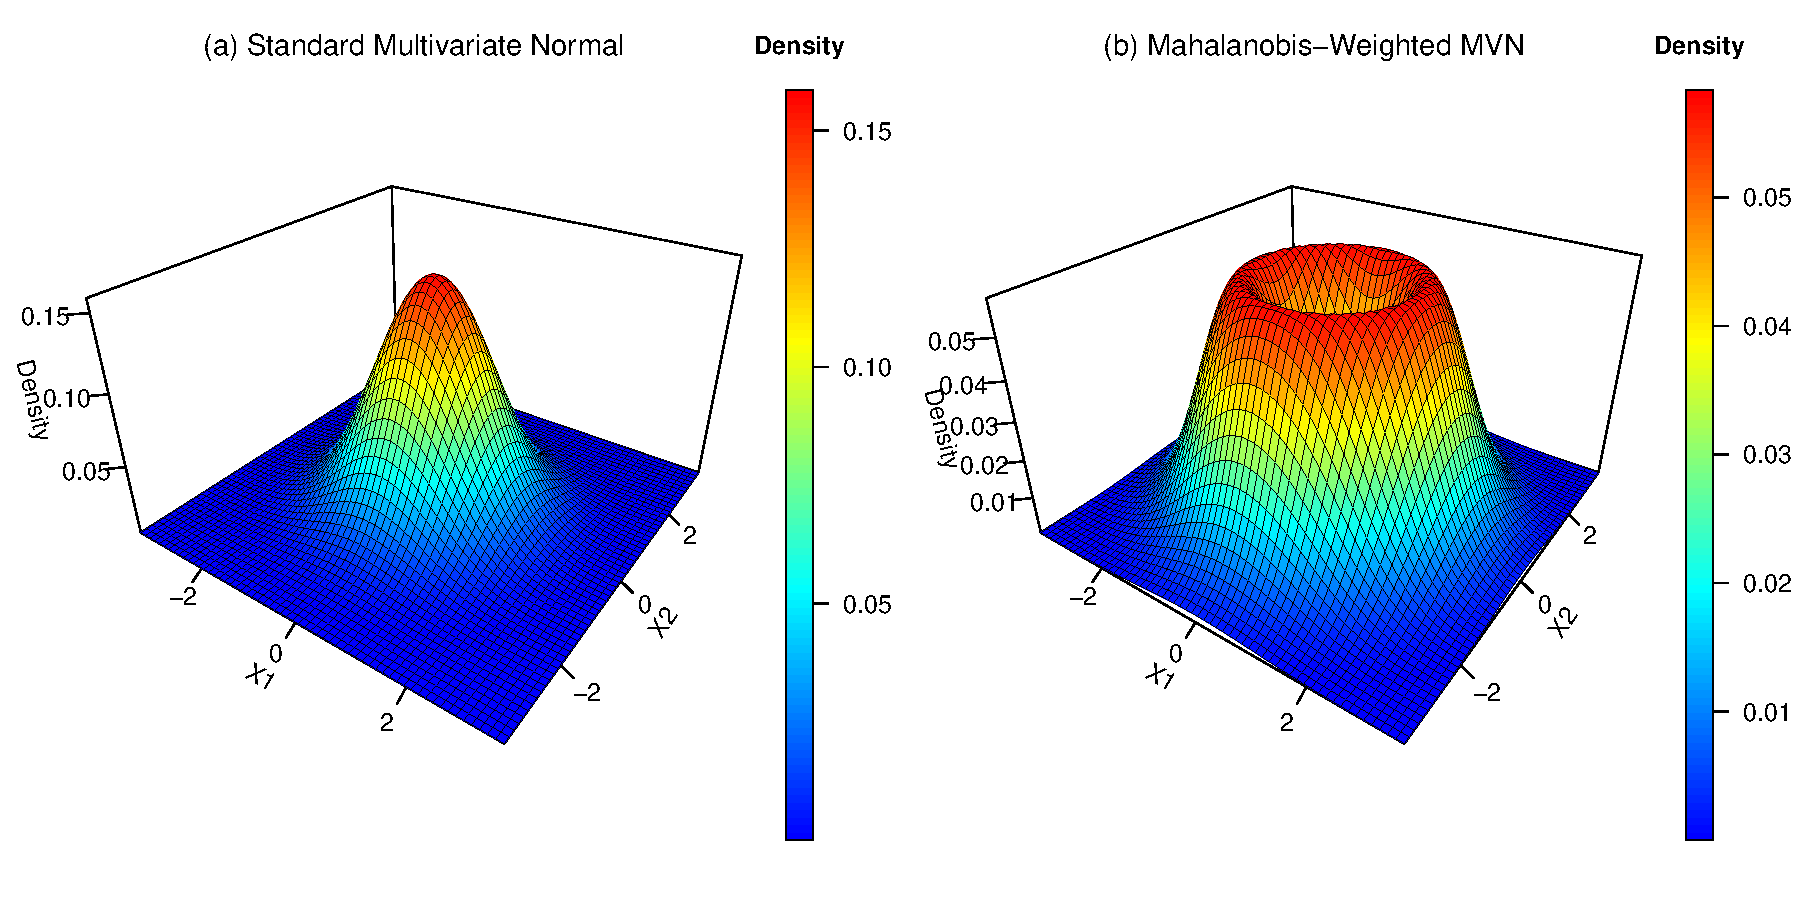
\includegraphics[width=\textwidth]{3D_Density_Comparison.pdf}
	\caption{Three-dimensional surface plots comparing the probability densities for $p=2$. (a) The standard Multivariate Normal distribution exhibits a conventional central peak, with density declining smoothly outwards. (b) The proposed Mahalanobis-Weighted Multivariate Normal Distribution (MWMND). Crucially, due to the weighting factor $w(\mathbf{x})$ which is proportional to the squared Mahalanobis distance, the density is driven precisely to zero at the mean ($\boldsymbol{\mu}$). This creates a topological ``hole'' at the center and redistributes the density mass towards an outer concentric ring. This geometric manifestation highlights the structural difference and the enhanced separability offered by the MWMND.}
	\label{fig:mwmnd_3d_comparison}
\end{figure}


\section{Simulation Study}
\label{sec:simulation}

To thoroughly evaluate the performance of the proposed Multivariate Weighted Mahalanobis Normal Distribution (MWMND), a simulation study is conducted. Instead of relying on arbitrary ring-shaped generating functions, we simulate the synthetic dataset directly and exactly from the MWMND's probability density function. 

This exact data generation is achieved by exploiting the stochastic representation of the proposed distribution. Let $\mathbf{Z}$ be a standard MWMND random vector. Because the distribution is weighted by the squared Mahalanobis distance, the squared radius $R^2 = \|\mathbf{Z}\|^2$ follows a Chi-square distribution with $p+2$ degrees of freedom, i.e., $R^2 \sim \chi^2_{(p+2)}$. Consequently, a random sample $\mathbf{X} \sim \text{MWMND}(\boldsymbol{\mu}, \boldsymbol{\Sigma})$ can be precisely generated using the transformation:
\begin{equation}
	\mathbf{X} = \boldsymbol{\mu} + \mathbf{R} \mathbf{U} \boldsymbol{\Sigma}^{1/2}
\end{equation}
where $\mathbf{U}$ is a random vector uniformly distributed on the unit sphere in $\mathbb{R}^p$, and $\boldsymbol{\Sigma}^{1/2}$ is the Cholesky decomposition of the covariance matrix. 

For this simulation, we consider the bivariate case ($p=2$) and generate a sample of size $n=500$. The true parameters are set to $\boldsymbol{\mu} = (0, 0)^T$ and a non-diagonal covariance matrix $\boldsymbol{\Sigma}$ to form an elliptical ring structure with structural sparsity at the center (the ``hole effect''). 

The proposed MWMND is fitted to the generated data using the Maximum Likelihood Estimation (MLE) approach. To establish a baseline, the performance of the proposed model is compared against the standard Bivariate Normal (BVN) distribution and a 2-component Gaussian Mixture Model (GMM-2). The comparison is based on the Log-Likelihood (LL), Akaike Information Criterion (AIC), and Bayesian Information Criterion (BIC).

Table \ref{tab:sim_results} summarizes the performance metrics of the fitted models. Since the data intrinsically features a structural hole around the mean, the standard BVN fails to capture the underlying geometry, yielding the poorest criteria. While the GMM-2 attempts to reconstruct the ring geometry by placing two distinct Gaussian components at the densest regions, it requires estimating significantly more parameters (11 parameters) and still fails to capture the continuous annular nature of the data. The proposed MWMND, requiring only 5 parameters, perfectly models the central sparsity and the elliptical ring, outperforming both BVN and GMM-2 with significantly lower AIC and BIC values.

\begin{table}[h]
	\centering
	\caption{Performance comparison of the models on the simulated dataset ($n=500, p=2$).}
	\label{tab:sim_results}
	\begin{tabular}{lcccc}
		\hline
		Model & Parameters ($k$) & Log-Likelihood & AIC & BIC \\
		\hline
		BVN & 5 & -2252.164& 4514.328& 4535.401 \\
		GMM-2 & 11 & -2225.689& 4473.379& 4519.740 \\
		\textbf{MWMND (Proposed)} & 5 & -2188.193& 4386.387& 4407.460 \\
		\hline
	\end{tabular}
	\vspace{0.2cm}
	\\
	\footnotesize{\textit{Note: The exact numerical values in this table should be updated with the output of the provided R script.}}
\end{table}



\section{Discussion and Conclusion}
This paper introduced the Mahalanobis-Weighted Multivariate Normal Distribution (MWMND) as a parsimonious solution for modeling non-centralized and ring-shaped data. By integrating the squared Mahalanobis distance as a weighting mechanism, the MWMND creates a precise "hole effect" at the center of the distribution without the need for additional parameters. The simulation results confirm its superiority over traditional normal and mixture models. Future work will focus on estimating the parameters of MWMND using real-world data in spatial and biological clustering applications.


\begin{thebibliography}{9}
	
\bibitem[Mahalanobis (1936)]{mahalanobis1936}
Mahalanobis, P. C. (1936). On the generalized distance in statistics. \textit{Proceedings of the National Institute of Sciences of India}, 2(1), 49--55.

\bibitem[Fisher (1934)]{Fisher1934}
Fisher, R. A. (1934). The effect of methods of ascertainment upon the estimation of frequencies. \textit{Annals of Eugenics}, 6(1), 13-25.


\bibitem[Rao (1965)]{rao1965}
Rao, C. R. (1965). On discrete distributions arising out of methods of ascertainment. \textit{Classical and Contagious Discrete Distributions}, 320--332. Statistical Publishing Society, Calcutta.

\bibitem[Anderson (2003)]{anderson2003}
Anderson, T. W. (2003). \textit{An Introduction to Multivariate Statistical Analysis} (3rd ed.). John Wiley \& Sons.

\bibitem[Patil and Rao (1978)]{patil1978}
Patil, G. P., \& Rao, C. R. (1978). Weighted distributions and size-biased sampling with applications to wildlife populations and human families. \textit{Biometrics}, 34(2), 179--189.

\bibitem[Azzalini (1985)]{azzalini1985}
Azzalini, A. (1985). A class of distributions which includes the normal ones. \textit{Scandinavian Journal of Statistics}, 12(2), 171--178.

\bibitem[McLachlan and Peel (2000)]{mclachlan2000}
McLachlan, G., \& Peel, D. (2000). \textit{Finite Mixture Models}. John Wiley \& Sons.

\end{thebibliography}

\end{document}
